\documentclass{article}

\usepackage[margin=1in]{geometry}
\usepackage{amsmath}
\usepackage{spverbatim}
\usepackage{graphicx}

\begin{document}
	
\title{ESOF 322 - Homework 4}
\author{Nathan Stouffer and Kevin Browder}

\maketitle
\newpage

\section*{Exercise 1}

\subsection*{Part A}
\subsubsection*{Problem 1}
Question: What system did you download?\\\\
Solution: We downloaded RxJava which is the Reactive Extensions for the Java Virtual Machine.

\subsubsection*{Problem 2}
Question: What does it do?\\\\
Solution: This library allows you to use Reactive Extension in Java. Reactive extensions is used for asynchronous programming. This library allows you to do asynchronous programming in Java.

\subsubsection*{Problem 3}
Question: How many Lines of Code does it have? How did you calculate this?\\\\
Solution: This library has about 50,000 lines of code. We calculated this by cloning the repo to a local machine and then using the git ls-files command to determine the number of lines in the documentation (7856) and then determining the number of lines of code in the entire library (57,503) using ls-files with different parameters. We can then subtract the documentation and find that there are around 50,000 lines of source code.

\subsection*{Part B}
\subsubsection*{Problem 1}
Question: Capture the output of the tool\\\\
Solution: 
\begin{figure}[h]
	\centering
	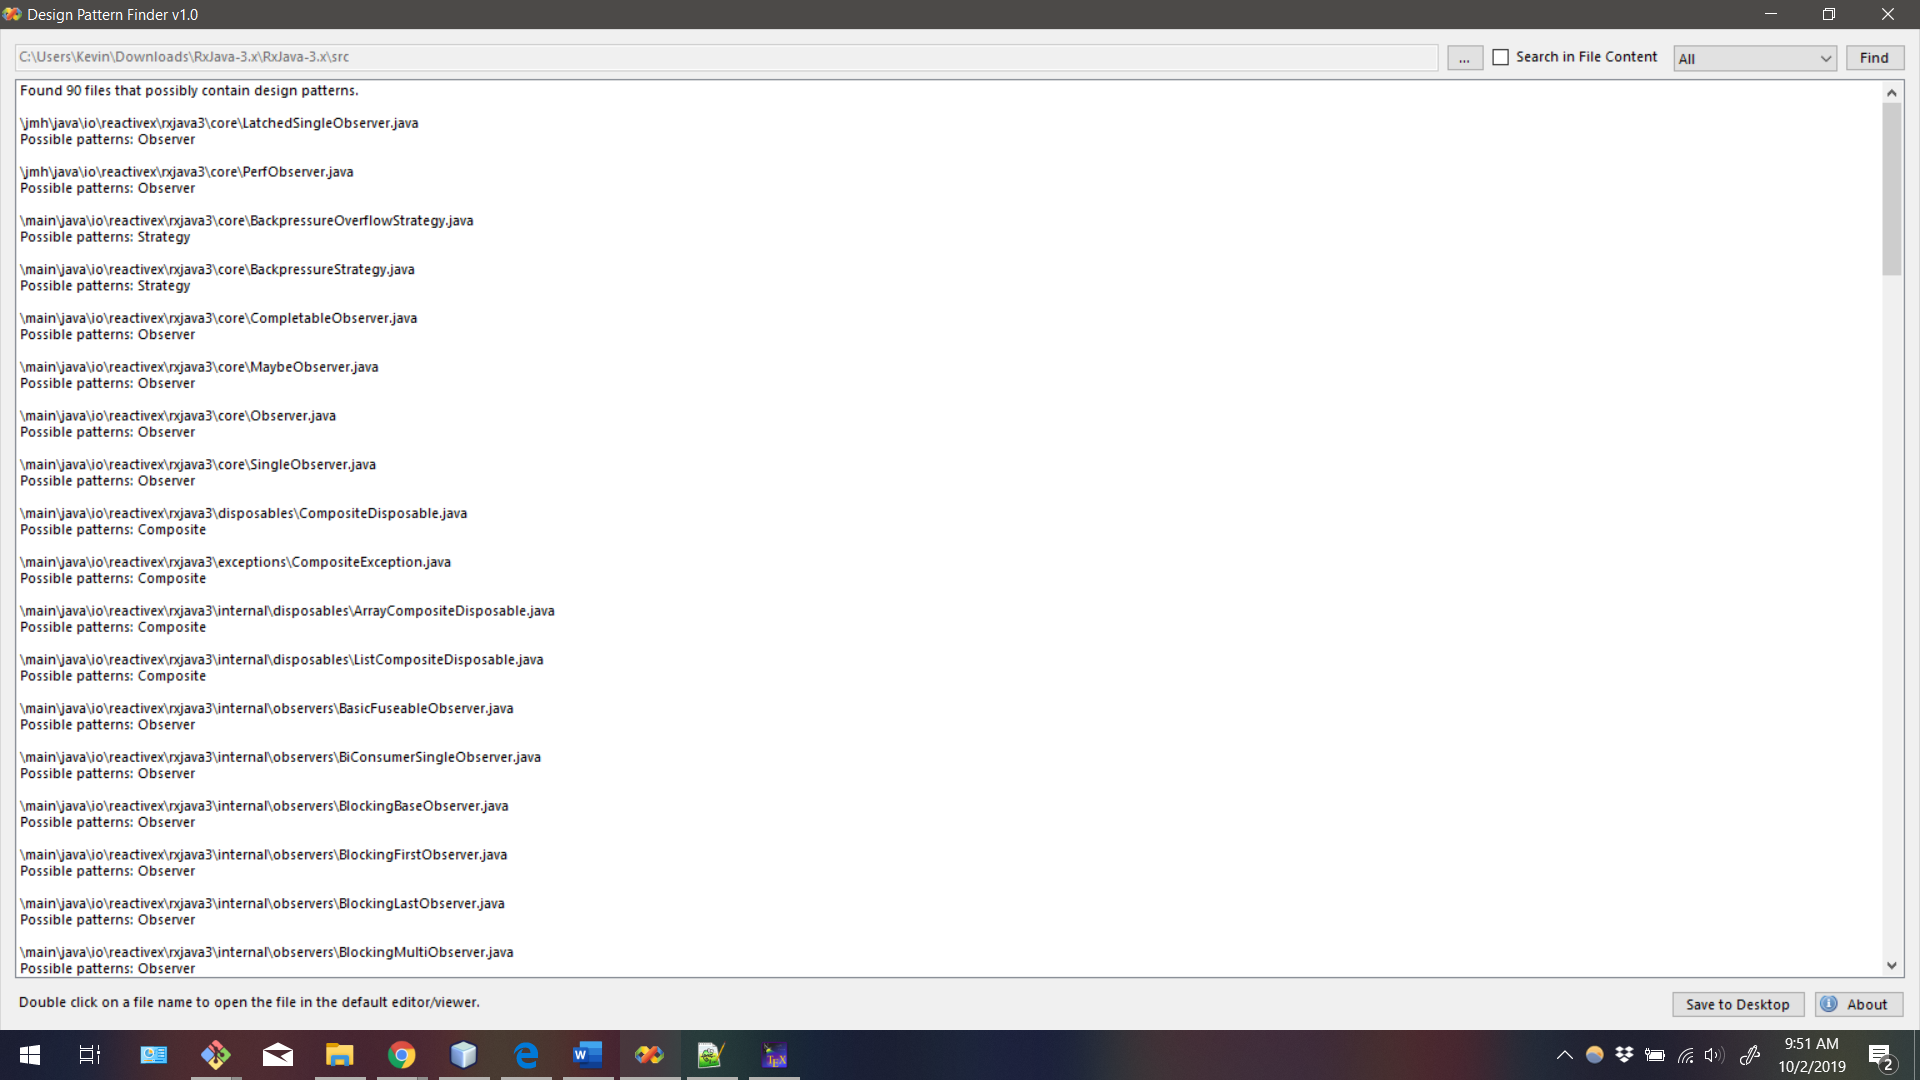
\includegraphics[width=6in]{hw4-patterns.png}
\end{figure}

\subsubsection*{Problem 2}
Question: How does the tool look for instances of the design pattern?\\\\
Solution: This program has a set of design pattern definitions in an xml file. It then starts iterating through the file structure and then through the code in each file comparing it to the definitions. If it finds a match it adds that pattern to the output. It then prints all the patterns it found in that file with the file path and then moves to the next file. 

\subsubsection*{Problem 3}
Question: Do you think the process used by the tool is correct?  How would you do it? Be specific\\\\
Solution: We would use a similar design to the DesignPatternTool. All of the design patterns have a distinct signature in code that can be defined. When a user gives a source code location the program could recursively go through every file in the structure beneath were the user defined to start. Each file could then be iterated through line by line and compared with the design pattern definitions supplied to it in the beginning. When it finds a match it would output the pattern it found and the file location. 

\newpage

\section*{Exercise 2}

\subsection*{Part A}
Problem: How did you upload the ESOF 322 files into your Github account? \\\\
Solution: We began by navigating to the esof-322 directory on my computer. We then created a local repository on my computer using the ``git init" command.
We then staged all the subdirectories in esof-322 for a commit. Next, we committed those files with the commit message ``initial commit".
Then, on our GitHub account, we created a repository called esof-322.
Finally, we set up the online repository as the remote for our local repository and pushed the initial commit.

\subsection*{Part B}
Problem: Add a file to the GitHub
Solution: The screenshot of the terminal while we added the file "hw-4-assignment.pdf" is shown below.
\begin{figure}[h]
	\centering
	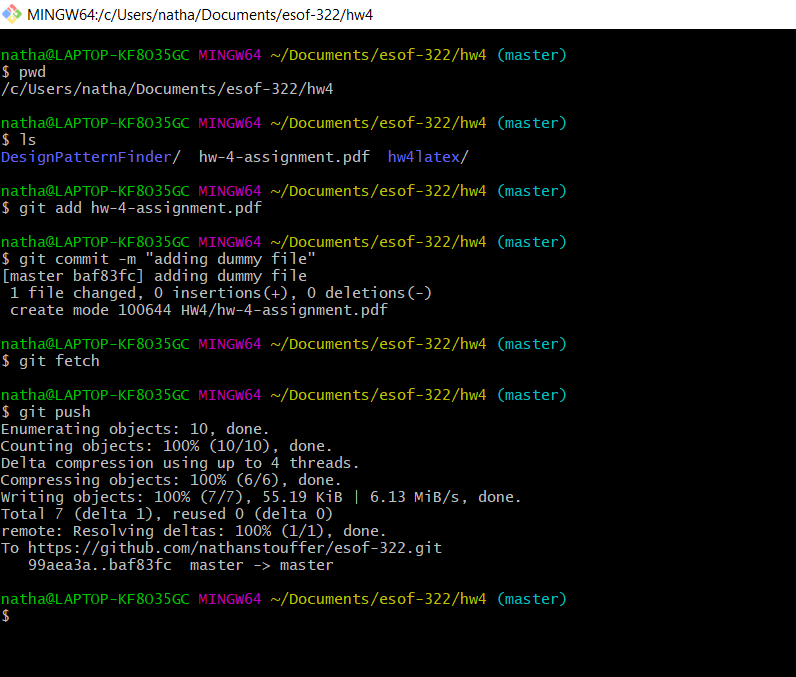
\includegraphics[width=5in]{dummy-file.jpg}
\end{figure}
\newpage
The figure below is proof that "hw-4-assignment.pdf" is in the repository on GitHub.
\begin{figure}[h]
	\centering
	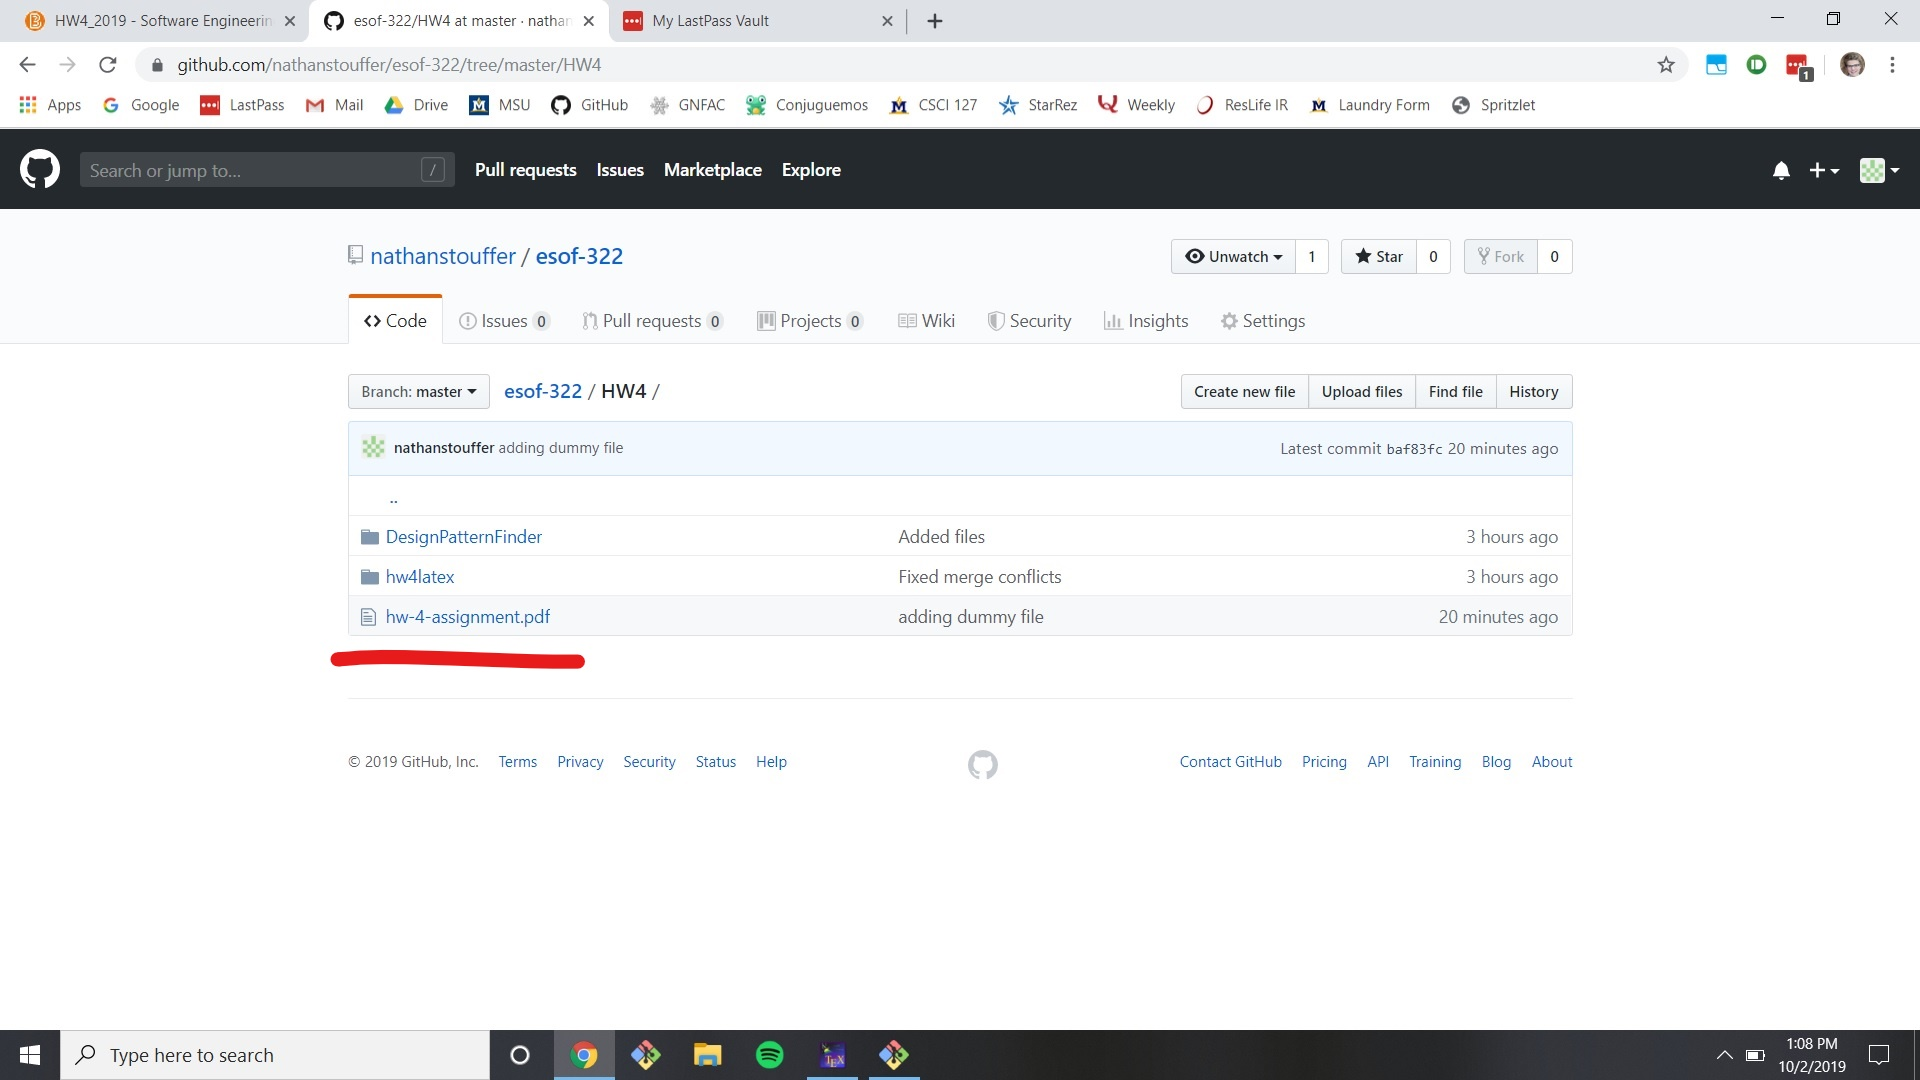
\includegraphics[width=5in]{dummy-file-on-GitHub.jpg}
\end{figure}


\end{document}